\title{Question 1}
\author{LJ Brown}
%\date{\today}

\documentclass[12pt]{article}
\usepackage{pgf, tikz}
\usetikzlibrary{arrows, automata}
\usepackage{amsmath}
\usepackage{blkarray}

\begin{document}
\maketitle

\section{Question}
1.	(25/25 points) Consider the following web pages and the set of web pages that they link to:
Page A points to pages B and C.
Page B points to page C.
All other pages have no outgoing links.
Apply the PageRank algorithm to this subgraph of pages. Assume $\alpha$ = 0.15. Simulate the algorithm for three iterations. 


% Web Graph
\begin{center}Web Graph \end{center}

\begin{center}
	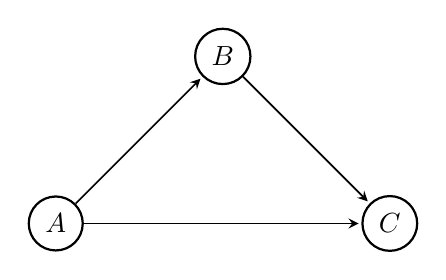
\begin{tikzpicture}[
            > = stealth, % arrow head style
            shorten > = 1pt, % don't touch arrow head to node
            auto,
            node distance = 3cm, % distance between nodes
            semithick % line style
        ]

        \tikzstyle{every state}=[
            draw = black,
            thick,
            fill = white,
            minimum size = 4mm
        ]

        \node[state] (A) {$A$};
        \node[state] (B) [above right of=A] {$B$};
        \node[state] (C) [below right of=B] {$C$};

        \path[->] (A) edge node {} (B);
        \path[->] (A) edge node {} (C);
        \path[->] (B) edge node {} (C);


        %\draw[red, dashed] (1, 2) -- (1, -2);
    \end{tikzpicture}
\end{center}


% Corrected Web Graph
\begin{center}Corrected Web Graph \end{center}

\begin{center}
	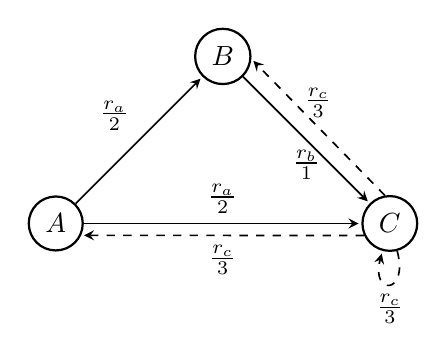
\begin{tikzpicture}[
            > = stealth, % arrow head style
            shorten > = 1pt, % don't touch arrow head to node
            auto,
            node distance = 3cm, % distance between nodes
            semithick % line style
        ]

        \tikzstyle{every state}=[
            draw = black,
            thick,
            fill = white,
            minimum size = 4mm
        ]

        \node[state] (A) {$A$};
        \node[state] (B) [above right of=A] {$B$};
        \node[state] (C) [below right of=B] {$C$};

        \path[->] (A) edge node {$\frac{r_a}{2}$} (B);
        \path[->] (A) edge node {$\frac{r_a}{2}$} (C);
        \path[->] (B) edge [align=center,below] node {$\frac{r_b}{1}$} (C);
        
        % added
        \path[->, dashed] (C) edge [loop below] node {$\frac{r_c}{3}$} (C);
        \path[->, dashed] (C.100) edge [align=center,above] node {$\frac{r_c}{3}$} (B.-5);
        \path[->, dashed] (C.205) edge node {$\frac{r_c}{3}$} (A.-25);

    \end{tikzpicture}
\end{center}

%Page rank for page $j$,
%\begin{equation}
%\nonumber r_j = \sum\limits_{i \in \left\{ {a, b, c, \, | i \rightarrow j} \right\}   } \frac{r_i}{d_i}
%\end{equation}
%where $d_i$ is the out degree of node $i$.

% flow equations
Flow Equations
\begin{equation}
	r_a = \frac{r_c}{3}
\end{equation}

\begin{equation}
	r_b = \frac{r_a}{2} + \frac{r_c}{3}
\end{equation}

\begin{equation}
	r_c = \frac{r_a}{2} + \frac{r_b}{1} + \frac{r_c}{3}
\end{equation}

% flow equations constraint
Flow Equations have no unique solution. 3 equations with 3 unknowns. Add additional constraint.

\begin{equation}
	r_a + r_b + r_c = 1
\end{equation}

Therefore if $alpha=0$,

\begin{equation}
	\nonumber r_a = \frac{2}{11}, \, r_b = \frac{3}{11}, \, r_c = \frac{6}{11}
\end{equation}

Which would correspond to the maximum right eigenvector of the matrix P below.

%
%	Link Matrix
%

Link Matrix,
\[
\begin{blockarray}{cccc}
a & b & c \\
\begin{block}{(ccc)c}
  0 & 1 & 1 & a \\
  0 & 0 & 1 & b \\
  0 & 0 & 0 & c \\
\end{block}
\end{blockarray}
\]

Row/Right Stochastic Transition Probability Matrix, $P$, 

$$
P = 
\left( 0.85 \right)
\begin{pmatrix} 
  0 	& \frac{1}{2} 	& \frac{1}{2}  \\
  0 	& 0 			& 1 		 \\
  \frac{1}{3} 	& \frac{1}{3} 	& \frac{1}{3}
\end{pmatrix}
 + 
\left( 0.15 \right)
\begin{pmatrix} 
  \frac{1}{3} 	& \frac{1}{3} 	& \frac{1}{3} \\
  \frac{1}{3} 	& \frac{1}{3} 	& \frac{1}{3} \\
  \frac{1}{3} 	& \frac{1}{3} 	& \frac{1}{3}
\end{pmatrix}
=
\begin{pmatrix} 
  0.05 	& 0.475 	& 0.475 \\
  0.05 	& 0.05 	& 0.09 \\
  0.33 \dots 	&  0.33 \dots 	&  0.33 \dots
\end{pmatrix}
$$




\end{document}